
\documentclass[conference]{IEEEtran}

%+++++++++++++++++++++++++++++++++++++++++++
% Added to commands
\input epsf
\usepackage{graphicx}
%\usepackage[labelformat=empty]{caption}
\usepackage{float}
%\usepackage{subcaption}
%\usepackage{flushend}
%\usepackage{balance}
\usepackage{amsmath}
\usepackage{mathtools}
%\usepackage{comment}
\setlength{\belowcaptionskip}{-8pt}
\usepackage [english]{babel}
\usepackage [autostyle, english = american]{csquotes}
\MakeOuterQuote{"}
%+++++++++++++++++++++++++++++++++++++++++++



% correct bad hyphenation here
\hyphenation{}
\begin{document}


\title{\LARGE \textbf{An MSER Approach to Tracking Multi-Agent Systems} \vspace{0ex}}

% make the title area
\maketitle

\section{Overview}

The computationally inexpensive detection of multiple features in an image or video frame presents an opportunity for the computational perception of multi-target and multi-agent systems. The Maximally Stable Extremal Regions (MSERs) technique has been shown to be a fast and robust way to detect multiple items in still images and video streams of complex scenes. As described in \cite{Matas02bmvc} and \cite{Donoser06cvpr}, the MSER method divides an input image into regions based on how the regions' brightness levels compare to a modifiable brightness threshold. "Maximally stable" regions are those whose shapes and dimensions change the least in response to changes in the brightness threshold. An advance in MSER algorithms developed by Nister and Stewenius \cite{Nister08eccv} allows MSERs to be computed in linear time with respect to the size of the input image. 

With robustness and computational efficiency, the MSER algorithm has great potential to perform in real-time as a general-purpose perception tool for use by mobile robots equipped with cameras. MSERs are essentially "blobs" in the input image that represent bright areas surrounded by darkness or dark areas surrounded by brightness. As a result, MSERs often correspond to visually distinguishable physical objects in the photographed environment. Figure \ref{fig:1} shows the results of the MSER computation as applied to an indoor scene. Note how objects in the indoor scene such as posters become highlighted by the MSER algorithm. 

\begin{figure}[ht]
\centering
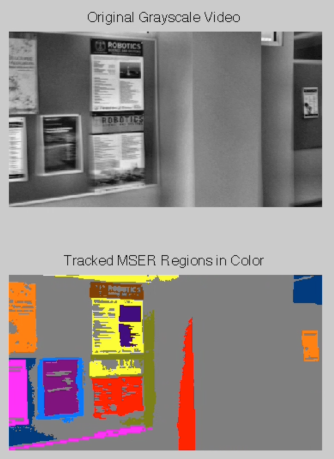
\includegraphics[width=0.3\textwidth]{MSER_Indoor.png}
\caption{Grayscale indoor image (top) with detected MSERs (bottom)}
\label{fig:1}
\vfill
\end{figure}

To be useful for robot navigation, perception of detected regions and their corresponding world objects must be persistent across robot video frames. For this purpose, a tracking technique is required. Tracking techniques specifically aimed at MSERs have been Developed by Donoser and Bischof in \cite{Donoser06cvpr} and \cite{Donoser10icpr}. Existing MSER tracking techniques keep track of a region from one video frame to another by first detecting the MSER in one frame, advancing to the next frame, and then re-performing the MSER technique in the general area of the MSER detected in the previous frame. Techniques such as this  rely on the assumption that the object represented by the region does not leave the frame and does not drastically change shape or position in between frames. Furthermore, these techniques are better suited for tracking a single region among others, not for tracking multiple regions simultaneously. The authors of these techniques to do not make any attempt at multi-agent or multi-target tracking. A further weakness of this approach is that there is no way to infer the position of the real-world object that gives rise to the detected MSER. One way to remedy the issues in existing MSER-based tracking techniques is to use a probabilistic inference approach. Specifically aimed at multi-agent problems, tracking techniques based on probabilistic inference have been proposed by Khan, Balch, and Dellaert in \cite{Khan06pami} and \cite{Khan05cvpr}. These probabilistic methods rely on a Rao-Blackwellized particle filter, a prediction equation that incorporates target dynamics information, and efficient Markov Chain Monte Carlo (MCMC) sampling. This technique achieved accurate tracking of many agents in a real-world video stream of ants, but did not incorporate the more recently advanced MSER techniques that make the tracking methods more generally applicable to robotic scene perception.  

In addition to being fast and robust, the MSER method is ideally suited to serve as a measurement input for the aforementioned probabilistic tracking techniques. Often described as a "blob detector" MSER identifies a groups  of pixels representing blobs in an image. As a result, the method can easily be extended to fit ellipses to the detected regions as shown in Figure \ref{fig:2}. Once a fitted ellipse is computed for each region, ellipse parameters such as center location and dimensions can serve as very compact measurement inputs to the probabilistic tracking techniques. Figure \ref{fig:3} shows a single image of multiple targets in the PyBioSim simulator and the resulting MSER ellipses.

\begin{figure}[ht]
\centering
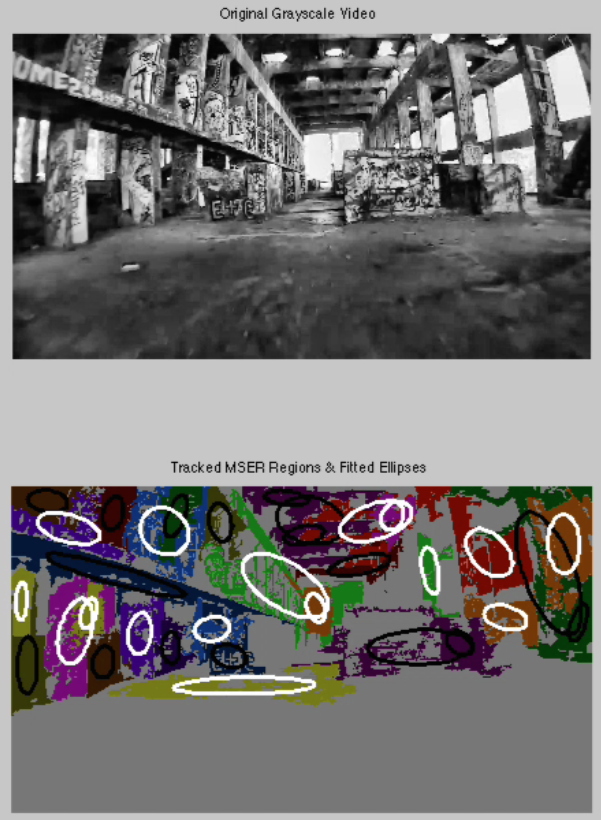
\includegraphics[width=0.3\textwidth]{Ellipses.png}
\caption{Grayscale indoor image (top) with detected MSERs and fitted ellipses (bottom). White ellipses correspond to bright MSERs with dark surroundings while black ellipses correspond to dark MSERs with bright surroundings.}
\label{fig:2}
\vfill
\end{figure} 

\begin{figure}[ht]
\centering
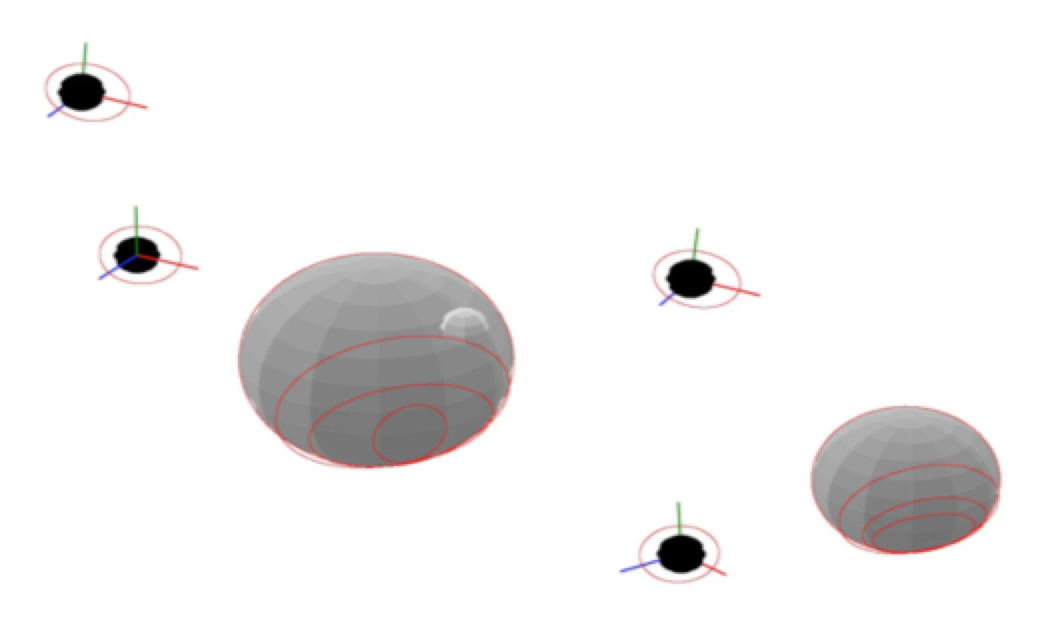
\includegraphics[width=0.3\textwidth]{Simulator.png}
\caption{Image from multiagent simulator with superimposed ellipses fitted to MSER region detection.}
\label{fig:3}
\vfill
\end{figure} 

\section{Research Question}

The goal of this work is to evaluate the use of MSER detection as an input to multi-target tracking methods. More specifically, an MSER-based multi-target tracking method will be prototyped and quantitatively evaluated to determine its viability. This goal is pursued because a successful MSER-based multi-target tracker could become a general-purpose scene understanding tool for mobile robots in complex environments that contain multiple objects and agents. 

\section{Implementation Approach}

This work will use a linear time implementation of MSERs to detect regions in a video stream extracted from the PyBioSim simulation environment. The locations of these regions will be used as measurement inputs to the implementation of the probabilistic inference method described in the previous section. Agents in the simulated environment will be programmed to move such that they occlude each other and add difficulty to the tracking operation.The tracking techniques will be used to infer 2D positions of the agents in the simulator.

\section{Quantitative Assessment}

Because the simulated environment produces precisely known ground truth information, the performance of the tracking method developed in this work will be measured using quantitative evaluation methods described in \cite{Bernadin08eurasip} by comparing the ground truth locations of the objects in the simulator with the inferred locations of the objects. \cite{Bernadin08eurasip} provides equations for computing multi-target tracking performance measures such as multiple object tracking precision, multiple object tracking accuracy, the number of false positives, the number of false negatives, and the number of mismatches. 

\section{Milestones}

\begin{enumerate}
  \item Implement MSER and PyBioSim pipeline that computes MSERs from PyBioSim video streams. Pipeline must include the correspondence between the positions in the video stream and positions in the MSER computation. 
  \item Implement particle filter based tracking method with MCMC sampling similar or identical to \cite{Khan06pami}.
  \item Implement \cite{Bernadin08eurasip} multi target tracking performance measure.
  \item Test the effectiveness of tracking and produce an analysis report.
\end{enumerate}

\section{Fallback}

The most difficult part of the implementation is the programming of the methods described in \cite{Khan06pami}. \cite{Khan06pami} is a very complex paper. As a result, if problems arise in the implementation of \cite{Khan06pami}, I will implement a simplified version. For example, I could implement only the particle filter instead of including MCMC sampling. A simple particle filter tracking algorithm is within my programming abilities and would still be a good way to test the combination of MSER methods and probabilistic tracking methods. 

\section*{Acknowledgments}

This work relies on the following freely available libraries:

\begin{itemize}
  \item PyBioSim (https://github.com/arindam1993/PyBioSim)
  \item GTSAM (tinyurl.com/gtsam)
  \item Linear Time MSER (https://github.com/idiap/mser)
  \item VL Feat (http://www.vlfeat.org)
  \item CLEAR MOT (https://github.com/smidm/clearmetrics)
\end{itemize}

\begin{thebibliography}{1}

\bibitem {Matas02bmvc} J. Matas, O Chum, M. Urban, and T. Pajdla, "Robust Wide Baseline Stereo from Maximally Stable Extremal Regions," \emph{Proceedings of British Machine Vision Conference,} pp. 384 - 396, 2002.

\bibitem {Donoser06cvpr} M. Donoser and H. Bischof, "Efficient Maximally Stable Extremal Region (MSER) Tracking," \emph{Proceedings of the 2006 IEEE Computer Society Conference on Computer Vision and Pattern Recognition (CVPR)}, 2006.

\bibitem {Nister08eccv} D. Nister and H. Stewenius, "Linear Time Maximally Stable Extremal Regions," \emph{10th European Conference on Computer Vision,} pp. 183 - 196, 2008.

\bibitem {Khan06pami} Z. Khan, T. Balch, and F. Dellaert, "MCMC Data Association and Sparse Factorization Updating for Real Time Multitarget Tracking with Merged and Multiple Measurements," \emph{IEEE Transactions on Pattern Analysis and Machine Intelligence (PAMI)}, pp. 1960 - 1971, 2006.

\bibitem {Khan05cvpr} Z. Khan, T. Balch, and F. Dellaert, "Multitarget Tracking with Split and Merged Measurements," \emph{Proceedings of the 2005 IEEE Computer Society Conference on Computer Vision and Pattern Recognition (CVPR)}, 2005.

\bibitem {Bernadin08eurasip} K. Bernadin and R. Stiefelhagen, "Evaluating Multiple Object Tracking Performance: The CLEAR MOT Metrics," \emph{EURASIP Journal on Image and Video Processing}, 2008.

\bibitem {Donoser10icpr} M. Donoser, H. Riemenschneider, and H. Bischof, "Shape Guided Maximally Stable Extremal Regions (MSER) Tracking," \emph{2010 International Conference on Pattern Recognition (ICPR),} pp. 1800 - 1803, 2010.

\end{thebibliography} 



\end{document}


 

